\let\negmedspace\undefined
\let\negthickspace\undefined
\documentclass[journal,12pt,onecolumn]{IEEEtran}
\usepackage{cite}
\usepackage{amsmath,amssymb,amsfonts,amsthm}
\usepackage{algorithmic}
\usepackage{graphicx}
\graphicspath{{./figs/}}
\usepackage{textcomp}
\usepackage{xcolor}
\usepackage{txfonts}
\usepackage{listings}
\usepackage{enumitem}
\usepackage{mathtools}
\usepackage{gensymb}
\usepackage{comment}
\usepackage{caption}
\usepackage[breaklinks=true]{hyperref}
\usepackage{tkz-euclide} 
\usepackage{listings}
\usepackage{gvv}                                          
\usepackage{xparse}
\usepackage{color}                                            
\usepackage{array}                                            
\usepackage{longtable}                                       
\usepackage{calc}                                             
\usepackage{multirow}
\usepackage{multicol}
\usepackage{hhline}                                           
\usepackage{ifthen}                                           
\usepackage{lscape}
\usepackage{tabularx}
\usepackage{array}
\usepackage{float}
\newtheorem{theorem}{Theorem}[section]
\newtheorem{problem}{Problem}
\newtheorem{proposition}{Proposition}[section]
\newtheorem{lemma}{Lemma}[section]
\newtheorem{corollary}[theorem]{Corollary}
\newtheorem{example}{Example}[section]
\newtheorem{definition}[problem]{Definition}
\newcommand{\BEQA}{\begin{eqnarray}}
	\newcommand{\EEQA}{\end{eqnarray}}
\newcommand{\define}{\stackrel{\triangle}{=}}
\theoremstyle{remark}
\newtheorem{rem}{Remark}

\newcommand{\ihat}{\mathbf {\hat \imath}}
\newcommand{\jhat}{\mathbf {\hat \jmath}}
\newcommand{\vect}[1]{\mathbf #1}



\title{CH: CHEMICAL ENGINEERING}
\author{EE25BTECH11042 - Nipun Dasari}
\date{   }


	
	\begin{document}
		
		\bibliographystyle{IEEEtran}
		\vspace{3cm}
		
		\maketitle
		

	
	\begin{enumerate}
		\item The number of emails received on six consecutive days is 11, 9, 18, 18, 4 and 15, respectively. 
		What are the median and the mode for these data?
		\begin{enumerate}
			\item  18 and 11, respectively
			\item  13 and 18, respectively
			\item  13 and 12.5, respectively
			\item  12.5 and 18, respectively
		\end{enumerate} 
		
		\item For two rolls of a fair die, the probability of getting a 4 in the first roll and a number less than 4 in 
		the second roll, up to 3 digits after the decimal point, is  \underline{\hspace{2cm}} 
		
		\item Which of the following statements are TRUE?
		\begin{enumerate}
			
			\item[(P.)] The eigenvalues of a symmetric matrix are real
			\item[(Q.)] The value of the determinant of an orthogonal matrix can only be +1
			\item[(R.)] The transpose of a square matrix A has the same eigenvalues as those of A
			\item[(S.)] The inverse of an $n\times n$ matrix exists if and only if the rank is less than n
		
		\end{enumerate}
		\begin{enumerate}
			\begin{multicols}{4}
	\item  P and Q only
	\item  P and R only
	\item  Q and R only
	\item  P and S only
		\end{multicols}
		\end{enumerate}
		\item Evaluate $\int \frac{dx}{e^x-1}$
		\begin{enumerate}
			\begin{multicols}{2}
	\item  $\frac{e^x}{e^x-1} +C$
	\item  $\frac{ln\brak{e^x - 1}}{e^x}$ + C
	\item  ln\brak{\frac{e^x}{e^x-1}} + C
	\item  ln\brak{1-e^-x} +C
			\end{multicols}
\end{enumerate} 
 \item A gaseous system contains H2, I2, and HI, which participate in the gas-phase reaction \\
 2 HI $\rightleftharpoons$ $H_2 +I_2$ \\
 At a state of reaction equilibrium, the number of thermodynamic degrees of freedom is \underline{\hspace{2cm}}

 \item The thermodynamic state of a closed system containing a pure fluid changes from \brak{T_1, p_1} to
 \brak{T_2, p_2}, where T and p denote the temperature and pressure, respectively. Let Q denote the heat
 absorbed \brak{> 0 \text{if absorbed by the system}} and W the work done \brak{> 0 \text{if done by the system}}. Neglect
 changes in kinetic and potential energies. Which one of the following is CORRECT?
  \begin{enumerate}
 	\item  Q is path-independent and W is path-dependent
 	\item  Q is path-dependent and W is path-independent
 	\item  is path-independent
 	\item   is path-independent
 \end{enumerate}
 
 \item An equation of state is explicit in pressure p and cubic in the specific volume v. At the critical point
 ‘c’, the isotherm passing through ‘c’ satisfies
   \begin{enumerate}
   \begin{multicols}{2}
 	\item  $\frac{\delta p}{\delta v} < 0$,$\frac{\delta^2p}{\delta v^2} = 0$
 	\item  $\frac{\delta p}{\delta v} > 0$,$\frac{\delta^2p}{\delta v^2} < 0$
 	\item  $\frac{\delta p}{\delta v} = 0$,$\frac{\delta^2p}{\delta v^2} > 0$
 	\item  $\frac{\delta p}{\delta v} = 0$,$\frac{\delta^2p}{\delta v^2} = 0$
 \end{multicols}
 \end{enumerate}
 
 \item The units of the isothermal compressibility are
    \begin{enumerate}
    	\begin{multicols}{2}
 	\item  $m^{-3}$
 	\item  $Pa^{-1}$
 	\item  $m^3Pa^-1$
 	\item  $m^{-3}Pa^{-1}$
 \end{multicols}
 \end{enumerate}
 
 \item An open tank contains two immiscible liquids of densities \brak{800 kg/m^3 \text{and} 1000 kg/m^3} as shown in
 the figure. If g = 10 m/$s^2$ , under static conditions, the gauge pressure at the bottom of the tank in Pa
 is  \underline{\hspace{2cm}}
 \begin{figure}[H]
 	\centering
 	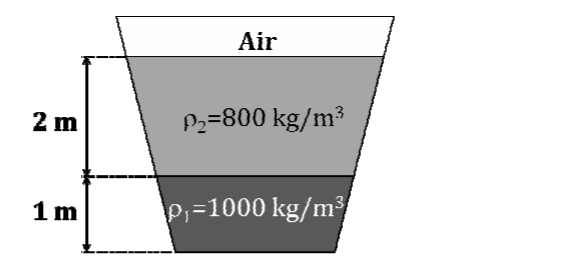
\includegraphics[width = 0.8\columnwidth]{q9.png}
 	\caption*{}
 	\label{fig:q9}
 \end{figure}

 \item The apparent viscosity of a fluid is given by \\
 0.007$|\frac{dV}{dy}|^{0.3}$, where \brak{\frac{dV}{dy}} is the velocity gradient. The fluid is:
      \begin{enumerate}
      	\begin{multicols}{2}
 	\item  Bingham plastic
 	\item  dilatant
 	\item  pseudoplastic
 	\item  thixotropic
 \end{multicols}
 \end{enumerate}
 
 \item The mass balance for a fluid with density $\rho$  velocity vector $\vec V$ is
       \begin{enumerate}
       	\begin{multicols}{2}
 	\item  $\frac{\delta p}{\delta t} + \Delta.\rho\vect{V}$
 	\item  $\frac{\delta p}{\delta t} + \rho.\Delta\vect{V}$
 	\item  $\frac{\delta p}{\delta t} + \vect{V}\Delta.\rho$
 	\item  $\frac{\delta p}{\delta t} -\vect{V} \Delta.\rho$
 \end{multicols}
 \end{enumerate}
 
 \item An incompressible Newtonian fluid, filled in an annular gap between two concentric cylinders of
 radii $R_1 and R_2$ as shown in the figure, is flowing under steady state conditions. The outer cylinder
 is rotating with an angular velocity of $\ohm$ while the inner cylinder is stationary. Given that
 \brak{R_2 - R_1} << $R_1 $the profile of the $\theta$-component of the velocity $V_\theta$ can be approximated by,
 \begin{figure}[H]
 	\centering
 	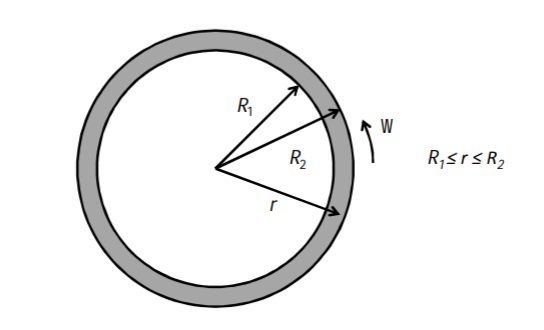
\includegraphics[width = 0.8\columnwidth]{q12.png}
 	\caption*{}
 	\label{fig:q12}
 \end{figure}
        \begin{enumerate}
        	\begin{multicols}{2}
 	\item  $R_2\ohm$
 	\item  $\frac{\brak{r-R_2}}{R_2-R_1}$
 	\item  $\frac{\brak{r+R_1}}{R_2+R_1}$
 	\item  $\frac{\brak{r-R_1}}{R_2-R_1}$
 \end{multicols}
 \end{enumerate}
 
 \item For a Newtonian fluid flowing in a circular pipe under steady state conditions in fully developed
 laminar flow, the Fanning friction factor is
         \begin{enumerate}
         	\begin{multicols}{2}
 	\item  $0.046Re^{-0.2}$
 	\item  $0.0014 + \frac{0.125}{Re^{0.32}}$
 	\item  $\frac{16}{Re}$
 	\item  $\frac{24}{Re}$
 \end{multicols}
 \end{enumerate} 
 
 \item In the Tyler standard screen scale series, when the mesh number increases from 3 mesh to 10 mesh,
 then
          \begin{enumerate}
          	\begin{multicols}{2}
 	\item  the clear opening decreases
 	\item  the clear opening increases
 	\item  the clear opening increases
 	\item  the clear opening increases
 \end{multicols}
 \end{enumerate} 
 
 \item Taking the acceleration due to gravity to be 10 m/$s^2$
 
 , the separation factor of a cyclone 0.5 m in
 
 diameter and having a tangential velocity of 20 m/s near the wall is  \underline{\hspace{2cm}}

 \item The effectiveness of a heat exchanger in the $\epsilon$-NTU method is defined as
            \begin{enumerate}
            	\begin{multicols}{2}
 	\item $\frac{{\brak{\text{increase in temperature of the cold fluid}}}}{{\brak{\text{decrease in temperature of the hot fluid}}}}$
 	\item  $\frac{{\brak{\text{actual exit temperature attained by the cold fluid}}}}{{\brak{\text{maximum exit temperature attainable by the cold fluid}}}}$
 	\item  $\frac{{\brak{\text{actual exit temperature attained by the hot fluid}}}}{{\brak{\text{minimum exit temperature attainable by the hot fluid}}}}$
 	\item  $\frac{{\brak{\text{actual heat transfer rate}}}}{{\brak{\text{maximum possible heat transfer rate from hot fluid to cold fluid}}}}$
 \end{multicols}
 \end{enumerate}
 
 \item In a pool boiling experiment, the following phenomena were observed.
 
 \begin{itemize}
 	\item[P.] Natural convention
 	\item[Q.] Film boiling
 	\item[R.] Transition boiling
 	\item[S.] Nucleate boiling
 \end{itemize}
 
 What was the CORRECT sequence of their occurrence?
             \begin{enumerate}
             	\begin{multicols}{2}
 	\item  P, Q, R, S
 	\item  S, R, Q, P
 	\item  Q, R, P, S
 	\item  P, S, R, Q
 \end{multicols}
 \end{enumerate}
 
 \item A hole of area 1 cm
 2
 is opened on the surface of a large spherical cavity whose inside temperature
 is maintained at 727 °C. The value of Stefan-Boltzmann constant is $5.67×10^-8 W/m^2-K^4$.
 Assuming black body radiation, the rate at which the energy is emitted \brak{\text{in W}} by the cavity through
 the hole, up to 3 digits after the decimal point, is  \underline{\hspace{2cm}}
 
 \item The packing of an existing absorption tower is replaced with a new type of packing. The height of
 the packing and the inlet conditions are maintained the same as before. Tests reveal that the
 number of transfer units is lower than before. This indicates that the tower with the new packing,
 when compared to that with the old packing, will
              \begin{enumerate}
              	\begin{multicols}{2}
 	\item  have a higher rate of absorption of the solute from the gas stream
 	\item  have a lower rate of absorption of the solute from the gas stream
 	\item  have the same rate of absorption of the solute from the gas stream
 	\item  have a lower height of transfer unit
 \end{multicols}
 \end{enumerate}
 
 \item A wet solid is dried over a long period of time by unsaturated air of nonzero constant relative
 humidity. The moisture content eventually attained by the solid is termed as the
               \begin{enumerate}
               	\begin{multicols}{2}
 	\item  have a lower height of transfer unit
 	\item  bound moisture content
 	\item  free moisture content
 	\item  equilibrium moisture content
 \end{multicols}
 \end{enumerate}
 
 \item The exit age distribution for a reactor is given by E\brak{t} = $\delta$\brak{t - 4}, where t is in seconds. A first order
 liquid phase reaction ($k = 0.25 s^-1$ ) is carried out in this reactor under steady state and isothermal
 conditions. The mean conversion of the reactant at the exit of the reactor, up to 2 digits after the
 decimal point, is  \underline{\hspace{2cm}}
 
 \item An isothermal liquid phase zero order reaction A $\rightarrow$ B (k = 0.5 mol/m3
 
 -s) is carried out in a batch
 
 reactor. The initial concentration of A is 2 mol/m3
 
 . At 3 seconds from the start of the reaction, the
 
 concentration of A in mol/m3
 
 is  \underline{\hspace{2cm}}
 
 \item The overall rates of an isothermal catalytic reaction using spherical catalyst particles of diameters
 1 mm and 2 mm are $r_{A1}$ and $r_{A2}$ (in $mol (kg-catalyst)^{-1} h^{-1}$
 ), respectively. The other physical
 properties of the catalyst particles are identical. If pore diffusion resistance is very high, the ratio
 $r_{A2}/r_{A1}$ is  \underline{\hspace{2cm}}
 
 \item In the manufacture of sulphuric acid by the contact process, the catalytic oxidation of SO2 is carried
 out in multiple stages mainly to 
                \begin{enumerate}
                	\begin{multicols}{2}
 	\item  increase the reaction rate by providing inter-stage heating
 	\item  increase the overall conversion by providing inter-stage heating
 	\item  increase the overall conversion by providing inter-stage cooling
 	\item  decrease the overall conversion by removing sulphur trioxide between stages
 \end{multicols}
 \end{enumerate}
 
 \item Match the following.
 \begin{tabular}{c c}
 	\textbf{Group 1} & \textbf{Group 2} \\
 	(P) Viscosity & (1) Pyrometer \\
 	(Q) Pressure & (2) Hot wire anemometer\\
 	(R) Velocity & (3) Rheometer\\
 	(S) Temperature & (4) Piezoelectric element 
 	 	
 \end{tabular}
                 \begin{enumerate}
                 	\begin{multicols}{2}
 	\item  P-4, Q-3, R-1, S-2
 	\item  P-3, Q-4, R-2, S-1
 	\item  P-3, Q-4, R-1, S-2
 	\item  P-4, Q-3, R-2, S-1
 \end{multicols} 
 \end{enumerate}
 
 
 
 \item For the function \\
 $f(z)= \frac{1}{(2-z)(z+2)}$ \\
 
 the residue at z = 2 is  \underline{\hspace{2cm}}
 
 \item The solution of the differential equation \\ 
 \begin{align*}
 	\frac{dy}{dx} - y^2 = 0,
 \end{align*}
 given y=1 and x=0 is
                  \begin{enumerate}
                  	\begin{multicols}{2}
 	\item  $\frac{1}{1+x}$
 	\item  $\frac{1}{1-x}$
 	\item  $\frac{1}{\brak{1-x}^2}$
 	\item  $\frac{x^3}{3} + 1$
 \end{multicols}
 \end{enumerate}
 
 \item The solution of the differential equation \\
  \begin{align*}
 	\frac{d^2y}{dx^2} - \frac{dy}{dx} + 0.25y = 0,
 \end{align*}
 given $\frac{dy}{dx}$ = 1 at x=0 is
                   \begin{enumerate}
                   	\begin{multicols}{2}
 	\item  $xe^{0.5x}-xe^{-0.5x}$
 	\item  $0.5xe^{x}-xe^{-x}$
 	\item  $xe^{0.5x}$
 	\item  $-xe^{0.5x}$
 \end{multicols}
 \end{enumerate}
 
 \item The value of the integral \\

 evaluated by Simpson’s rule using 4 subintervals (up to 3 digits after the decimal point) is \underline{\hspace{2cm}}
 
 \item In a process occurring in a closed system F, the heat transferred from F to the surroundings E is
 600 J. If the temperature of E is 300 K and that of F is in the range 380 - 400 K, the entropy
 changes of the surroundings ($\delta S_E$) and system ($\delta S_F$), in J/K, are given by
                    \begin{enumerate}
                    	\begin{multicols}{2}
 	\item  $\Delta_E = 2$, $\Delta_F = -2$
 	\item  $\Delta_E = -2$, $\Delta_F = 2$
 	\item  $\Delta_E = 2$, $\Delta_F = -2$
 	\item  $\Delta_E = 2$, $\Delta_F = -2$
 \end{multicols}
 \end{enumerate}
 
 \item A binary liquid mixture is in equilibrium with its vapor at a temperature T = 300 K. The liquid
 mole fraction $x^1$ of species 1 is 0.4 and the molar excess Gibbs free energy is 200 J/mol. The value
 of the universal gas constant is 8.314 J/mol-K, and $\gamma_i$ denotes the liquid-phase activity coefficient of
 species i. If ln\brak{\gamma_1} = 0.09, then the value of ln\brak{\gamma_2}, up to 2 digits after the decimal point, is  \underline{\hspace{2cm}}
 
 \item Water \brak{density= 1000 kg/m^3} is flowing through a nozzle, as shown below and exiting to the
 atmosphere. The relationship between the diameters of the nozzle at locations 1 and 2 is $D_1 = 4 D_2$.
 The average velocity of the stream at location 2 is 16 m/s and the frictional loss between location 1
 and location 2 is 10000 Pa. Assuming steady state and turbulent flow, the gauge pressure in Pa, at
 location 1 is  \underline{\hspace{2cm}}
 
 \begin{figure}[H]
 	\centering
 	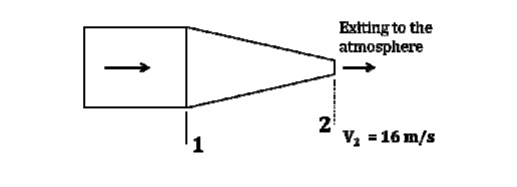
\includegraphics[width = 0.8\columnwidth]{q32.png}
 	\caption*{}
 	\label{fig:q32}
 \end{figure}
 
 \item In the elutriation leg of a commercial crystallizer containing a mixture of coarse and very fine
 crystals of the same material, a liquid is pumped vertically upward. The liquid velocity is adjusted
 such that it is slightly lower than the terminal velocity of the coarse crystals only. Hence
                     \begin{enumerate}
                     	\begin{multicols}{2}
 	\item  the very fine and coarse crystals will both be carried upward by the liquid
 	\item  the very fine and coarse crystals will both settle at the bottom of the tube
 	\item  the very fine crystals will be carried upward and the coarse crystals will settle
 	\item  the coarse crystals will be carried upward and the very fine crystals will settle
 \end{multicols}
 \end{enumerate}
 
 \item 100 ton/h of a rock feed, of which 80\% passed through a mesh size of 2.54 mm, were reduced in
 size such that 80\% of the crushed product passed through a mesh size of 1.27 mm. The power
 consumption was 100 kW. If 100 ton/h of the same material is similarly crushed from a mesh size
 of 5.08 mm to a mesh size of 2.54 mm, the power consumption \brak{\text{in kW, to the nearest integer}} using
 Bond’s law, is  \underline{\hspace{2cm}}
 
 \item Calculate the heat required \brak{\text{in kJ, up to 1 digit after the decimal point}} to raise the temperature of
 1 mole of a solid material from 100 °C to 1000 °C. The specific heat \brak{C_p} of the material \brak{\text{in
 J/mol-K}} is expressed as $C_p = 20 + 0.005T$, where T is in K. Assume no phase change.  \underline{\hspace{2cm}}
 
 \item In a double pipe counter-current heat exchanger, the temperature profiles shown in the figure were
 observed. During operation, due to fouling inside the pipe, the heat transfer rate reduces to half of
 the original value. Assuming that the flow rates and the physical properties of the fluids do not
 change, the LMTD \brak{\text{in} \degree C} in the new situation is
 
 \begin{figure}[H]
 	\centering
 	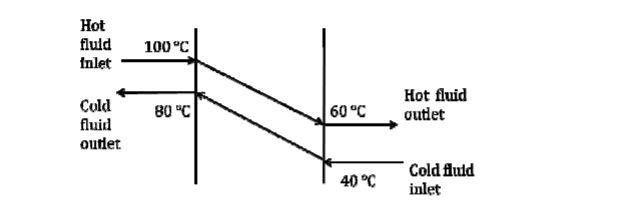
\includegraphics[width = 0.8\columnwidth]{q36.png}
 	\caption*{}
 	\label{fig:q36}
 \end{figure}
                      \begin{enumerate}
                      	\begin{multicols}{2}
 	\item  0
 	\item  20
 	\item  40
 	\item  indeterminate
 \end{multicols}
 \end{enumerate}
 
 \item The vapor-liquid equilibrium curve of a binary mixture A-B, may be approximated by a linear
 equation over a narrow range of liquid mole fractions $( 0.2 < x_A < 0.3)$ as follows \\ 
 
 \begin{align*}
 	y_A = 1.325x_A + 0.121
 \end{align*}
 
 Here $y_A$
 is the mole fraction of A in the vapor. 100 moles of a feed \brak{ x_{A,W} = 0.28} is batch distilled
 
 to a final residue \brak{x_{A,W} = 0.2}. Using the Rayleigh equation, the number of moles of the residue
 
 left behind in the distillation unit, up to 2 digits after the decimal point, is  \underline{\hspace{2cm}}
 
 
 \item A crosscurrent cascade of N ideal stages is used to treat a feed stream of molar flow rate E. The
 feed stream contains a solute which is to be recovered by a pure solvent having a molar flow rate S.
 The solvent is divided equally between these N stages. The linear equilibrium curve relating the
 mole fractions x and y* of the solute in the raffinate and the extract respectively, is given by
 y* = m x. Assume dilute conditions. The ratio of the solute mole fraction in the original feed to
 that in the exit raffinate stream i.e. \brak{x_0 / x_N}  is given by
                       \begin{enumerate}
                       	\begin{multicols}{2}
 	\item $\brak{1+\frac{mS}{NE}}^N$
 	\item  $\brak{1+\frac{NE}{mS}}^N$
 	\item  $\brak{1+\frac{NE}{mS}}^N$
 	\item  $\brak{1+\frac{mS}{NE}}^N$
 \end{multicols}
 \end{enumerate}
 
 \item A study was conducted in which water was pumped through cylindrical pipes made of a sparingly
 soluble solid. For a given pipe and certain flow conditions, the mass transfer coefficient $k_c$ has been
 calculated as 1 mm/s using the correlation \\ 
  \begin{align*}
 	Sh = 0.025 Re^{0.6} Sc^{0.33}
 \end{align*}
 If the velocity of the fluid and the diameter of the pipe are both doubled, what is the new value of $k_c$
 in mm/s, up to 2 digits after the decimal point?  \underline{\hspace{2cm}}
 
 
 \item The gas phase decomposition of azomethane to give ethane and nitrogen takes place according to
 the following sequence of elementary reactions.
 \begin{align*}
 (CH_3)_2N_2 + (CH_3)_2N_2 \overset{k_1}\rightarrow (CH_3)_2N_2 + [(CH_3)_2N_2]* \\
 [(CH_3)_2N_2]* + (CH_3)_2N_2 \overset{k_2}\rightarrow (CH_3)_2N_2 + (CH_3)_2N_2  \\
 [(CH_3)_2N_2]*  \overset{k_3}\rightarrow C_2H_6 +N_2
 \end{align*}
 
 Using the pseudo-steady-state-approximation for $[(CH_3)_2N2]*$, the order with respect to azomethane
 in the rate expression for the formation of ethane, in the limit of high concentrations of azomethane,
 is \underline{\hspace{2cm}}
 
 \item A first order liquid phase reaction is carried out isothermally at a steady state in a CSTR and 90%
 conversion is attained. With the same inlet conditions and for the same overall conversion, if the
 CSTR is replaced by two smaller and identical isothermal CSTRs in series, the \% reduction in total
 volume, to the nearest integer, is  \underline{\hspace{2cm}}
 
 \item Match the reactant-product combination in Group 1 with the unit process in Group 2. \\
  \begin{tabular}{c c}
 	\textbf{Group 1} & \textbf{Group 2} \\
 	(P) propylene- butanol & (1) Pyrolysis \\
 	(Q) cumene- phenol & (2) Dehydrogenation\\
 	(R) butane-butadiene & (3) Hydroformylation\\
 	(S) ethylene dichloride - vinyl chloride & (4) Peroxidation element 
 	
 \end{tabular}
 \begin{enumerate}
 	\begin{multicols}{2}
 	\item  P-3, Q-2, R-4, S-1
 	\item  P-2, Q-4, R-3, S-1
 	\item  P-1, Q-3, R-2, S-4 
 	\item  P-3, Q-4, R-2, S-1
 \end{multicols}
 \end{enumerate}
 
 \item Identify which of the following statements are FALSE.
 
 \begin{itemize}
 	\item[(P)]Oils with an oleic radical (1 double bond) are more suitable than oils with a linolenic radical
 	(3 double bonds) as film forming vehicles for paints
 	\item[(Q)] Production of synthesis gas from coal and steam is an endothermic process
 	\item[(R)]Use of chlorine for bleaching of wood pulp results in the release of dioxins
 	\item[(S)]In the manufacture of urea from ammonia, the main intermediate product formed is ammonium
 	bicarbonate
 \end{itemize}
 
  \begin{enumerate}
  	\begin{multicols}{2}
 	\item P and Q only   
 	\item  R and S only
 	\item  Q and R only 
 	\item P and S only 
 \end{multicols}
 \end{enumerate}
 
 \item A unit gain $2^{nd}$ order underdamped process has a period of oscillation 1 second and decay ratio
 0.25. The transfer function of the process is
   \begin{enumerate}
   	\begin{multicols}{2}
 	\item  $\frac{1}{0.024s^2 +0.067s + 1}$
 	\item  $\frac{1}{0.067s^2 +0.024s + 1}$
 	\item  $\frac{1}{0.021s^2 +0.1176s + 1}$
 	\item  $\frac{1}{0.1176s^2 +0.021s + 1}$
 \end{multicols}
 \end{enumerate}
 
 \item A control valve, with a turndown ratio of 50, follows equal percentage characteristics. The flow rate
 of a liquid through the valve at 40\% stem position is $1 m^3/h$. What will be the flow rate in $m^3$
 /h at 50\% stem position, if the pressure drop across the valve remains unchanged? \brak{\text{Up to 2 digits after
 the decimal point}}  \underline{\hspace{2cm}}
 
 \item The purchase cost of a heat exchanger of 20 $m^2$ 
 area was Rs. 500000 in 2006. What will be the 
 estimated cost \brak{\text{in Rs. to the nearest integer}} of a similar heat exchanger of 50 $m^2$
 area in the year 2013? Assume the six-tenths factor rule for scaling and the cost index for 2006 as 430.2. The
 projected cost index for the year 2013 is 512.6.  \underline{\hspace{2cm}}
 
 \item A plant manufactures compressors at the rate of N units/day. The daily fixed charges are Rs. 20000
 and the variable cost per compressor is Rs. 500 + 0.2 N
 1.3
 . The selling price per compressor is
 Rs. 1000. The number of compressors to be manufactured, to the nearest integer, in order to
 maximize the daily profit is  \underline{\hspace{2cm}}
 
  
 \textbf{Common Data for Questions 48 and 49:}
 
 A reverse osmosis unit treats feed water \brak{F} containing fluoride and its output consists of a permeate stream
 \brak{P} and a reject stream \brak{R}. Let $C_F, C_P, and C_R$ denote the fluoride concentrations in the feed, permeate, and
 reject streams, respectively. Under steady state conditions, the volumetric flow rate of the reject is 60 \% of
 the volumetric flow rate of the inlet stream, and $C_F$ = 2 mg/L and $C_P$ = 0.1 mg/L. 
 
 \item The value of CR in mg/L, up to one digit after the decimal point, is \underline{\hspace{2cm}}
 
\item A fraction f of the feed is bypassed and mixed with the permeate to obtain treated water having a
fluoride concentration of 1 mg/L. Here also the flow rate of the reject stream is 60\% of the flow rate
entering the reverse osmosis unit \brak{\text{after the bypass}}. The value of f , up to 2 digits after the decimal
point, is \underline{\hspace{2cm}}

\textbf{Common Data for Questions 50 and 51:}
Liquid reactant A decomposes as follows
\begin{align*}
	A\rightarrow R \hspace{2cm} r_R=k_1C_A^2 \hspace{2cm} k_1 = 0.5m^3/mol-s \\
	A\rightarrow S \hspace{2cm} k_2C_A \hspace{2cm} k_2 = 1s^-1
\end{align*}

An aqueous feed of composition$C_{A0} =30 mol/m^3$

, $C_{R0} = 2 mol/m^3$

, and $C_{S0}= 1 mol/m^3$

enters a CSTR in which the above reactions occur. Assume isothermal and steady state conditions.

\item If the conversion of A is 80 \%, the concentration of R in the exit stream in mol/$m^3$

, to the nearest

integer, is  \underline{\hspace{2cm}}

\item What is the \% conversion of A, to the nearest integer, so that the concentration of S in the exit stream is 11.8 mol/$m^3$?  \underline{\hspace{2cm}}



\textbf{Statement for Linked Answer Questions 52 and 53:} \\ 
The vapor liquid equilibrium relation for an ideal binary system is given by 
\begin{align*}
	y_A * = \frac{\alpha_{AB}\chi_A}{1+(\alpha_{AB}-1)\chi_A}
\end{align*}
Here $\chi_A$ and $y_A *$ are the mole fractions of species A in the liquid and vapor, respectively. The relative

volatility \brak{\alpha_{AB}}is greater than unity.

\item The liquid mole fraction $\chi_A$ at which the maximum difference between the equilibrium vapor mole
fraction and liquid mole fraction occurs is
   \begin{enumerate}
   	\begin{multicols}{2}
	\item  $\frac{1}{1+\sqrt{\alpha_{AB}}}$
	\item  $\frac{0.75}{1+\sqrt{\alpha_{AB}}}$
	\item  $\frac{0.5}{\sqrt{1+\alpha_{AB}}}$
	\item  $\frac{0.75}{\sqrt{1+\alpha_{AB}}}$
\end{multicols}
\end{enumerate}

\item A liquid having the composition found in the first part of the linked answer question, is flash
distilled at a steady state to a final liquid mole fraction of $0.25$. If $\alpha_{AB}$ is $2.5$, the fraction of the
feed vaporized is
   \begin{enumerate}
   	\begin{multicols}{2}
	\item $0.08$ 
	\item  $0.20$
	\item  $0.67$
	\item  $0.74$
\end{multicols}
\end{enumerate}

\textbf{Statement for Linked Answer Questions 54 and 55:} \\
 Consider the following transfer function
 \begin{align*}
 	G_p (s) = \frac{5}{(2s+1)^4}
 \end{align*}
 \brak{\text{Note: The unit of the process time constant is in seconds.}}
 
 \item The crossover frequency \brak{in rad/s} of the process is
    \begin{enumerate}
    	\begin{multicols}{2}
 	\item  $20$
 	\item  $0.1$
 	\item  $0.5$
 	\item $0.05$
 \end{multicols} 
 \end{enumerate}
 
 \item For the computation of Ziegler-Nichols settings, the ultimate period \brak{\text{in s/cycle}} and the ultimate
 gain are
     \begin{enumerate}
     	\begin{multicols}{2}
 	\item  $\pi and 0.8$
 	\item  $4\pi and 0.8$
 	\item  $4\pi and 1.25$
 	\item $\pi and 1.25$
 \end{multicols} 
 \end{enumerate}
 
 
 
 
 \item If 3 $\le$ X $\le$ 5 and 8 $\le$   Y $\le$  11  then which of the following options is TRUE?
      \begin{enumerate}
      	\begin{multicols}{4}
 	\item  $\frac{3}{5} \le \frac{X}{Y} \le \frac{8}{5}$
 	\item  $\frac{3}{11} \le \frac{X}{Y} \le \frac{5}{8}$
 	\item  $\frac{3}{11} \le \frac{X}{Y} \le \frac{8}{5}$
 	\item  $\frac{3}{5} \le \frac{X}{Y} \le \frac{8}{11}$
 \end{multicols}
 \end{enumerate}
 
 \item The Headmaster  \underline{\hspace{2cm}} to speak to you. \\
 Which of the following options is incorrect to complete the above sentence?
       \begin{enumerate}
       	\begin{multicols}{2}
 	\item  is wanting
 	\item  wants
 	\item  want
 	\item  was wanting
 \end{multicols}
 \end{enumerate}
 
 \item Mahatama Gandhi was known for his humility as
        \begin{enumerate}
        	\begin{multicols}{2}
 	\item   he played an important role in humiliating exit of British from India
 	\item  he worked for humanitarian causes
 	\item  he displayed modesty in his interactions
 	\item he was a fine human being
 \end{multicols} 
 \end{enumerate}
 
 \item \underline{All engineering students}$_\mathrm{I}$ \underline{should learn mechanics,}$_\mathrm{II}$ \underline{mathematics and}$_\mathrm{III}$\underline{how to do computation}$_\mathrm{IV}$ \\
 Which of the above underlined parts of the sentence is not appropriate?
         \begin{enumerate}
         	\begin{multicols}{2}
 	\item  I
 	\item  II
 	\item  III
 	\item  IV
 \end{multicols}
 \end{enumerate}
 \item Select the pair that best expresses a relationship similar to that expressed in the pair:
 water: pipe::
          \begin{enumerate}
          	\begin{multicols}{2}
 	\item cart: road  
 	\item  electricity: wire
 	\item   sea: beach
 	\item  music: instrument
 \end{multicols}
 \end{enumerate}
 
 \textbf{Q.61 to 65 carry two marks each.}
 
 \item Velocity of an object fired directly in upward direction is given by V = 80 - 32 t, where t is in seconds. When will velocity be between 
           \begin{enumerate}
           	\begin{multicols}{2}
 	\item  \brak{1,3/2}
 	\item  \brak{1/2,1}
 	\item  \brak{1/2,3/2}
 	\item  \brak{1,3}
 \end{multicols}
 \end{enumerate}
 
 \item In a factory, two machines M1 and M2 manufacture 60\% and 40\% of the autocomponents
 respectively. Out of the total production, 2\% of M1 and 3\% of M2 are found to be defective. If a
 randomly drawn autocomponent from the combined lot is found defective, what is the probability
 that it was manufactured by M2?
            \begin{enumerate}
            	\begin{multicols}{4}
 	\item  $0.35$
 	\item  $0.45$
 	\item  $0.5$
 	\item  $0.4$
 \end{multicols}
 \end{enumerate}
 
 \item Following table gives data on tourists from different countries visiting India in the year 2011.\\
 \begin{tabular}{|c|c|}
 \hline 
 \textbf{country} & \textbf{Number of Tourists} \\ \hline 
 USA & 2000 \\ \hline 
 England & 3500 \\ \hline 
 Germany & 1200 \\ \hline 
 Italy & 1100 \\ \hline 
 Japan & 2400 \\ \hline
 Australia & 2300 \\ \hline 
 France & 1000 \\ \hline  	
 \end{tabular} \\
 Which two countries contributed to the one third of the total number of tourists who visited India in
 2011?
             \begin{enumerate}
             	\begin{multicols}{2}
 	\item  USA and Japan
 	\item  USA and Australia
 	\item  England and France
 	\item  Japan and Australia
 \end{multicols}
 \end{enumerate}
 
 \item If $|-2X + 9|$ = 3 then the possible value of $|-X|$ -$X^2$ would be:
              \begin{enumerate}
              	\begin{multicols}{2}
 	\item  $30$
 	\item  $-30$
 	\item  $-42$
 	\item  $42$
 \end{multicols}
 \end{enumerate}
 
 \item All professors are researchers \\
 Some scientists are professors \\ 
 \\ 
 Which of the given conclusions is logically valid and is inferred from the above arguments:
               \begin{enumerate}
               	\begin{multicols}{2}
 	\item  All scientists are researchers
 	\item  All professors are scientists
 	\item  Some researchers are scientists
 	\item  No conclusion follows
 \end{multicols}
 \end{enumerate}
 
 
 

 
 

	\end{enumerate}
	\end{document}